\documentclass[]{msulabm}
\usepackage[utf8]{inputenc}
\usepackage{amsmath}
\usepackage{graphicx}
%\usepackage[linktocpage]{hyperref}  % if not using colorlinks, use linktocpage
\usepackage[colorlinks]{hyperref}  % if not using colorlinks, use linktocpage
\usepackage{bm}            % bold math
\usepackage{multirow}
\usepackage[table]{xcolor} % provide alternating rows with colors
\usepackage{textcomp}
\usepackage{xfrac} % gives split-level fractions with '\sfrac{a}{b}
\usepackage{multicol}
\usepackage[section]{placeins} % provides \FloatBarrier, to keep floats from crossing this barrier
\usepackage{amssymb}
\usepackage{wrapfig} % provides wrapping figures with text.
%\usepackage{enumitem} % gives \begin{enumerate}[resume] to resume counting from previous enumerate
%\usepackage{subfigure}
%\usepackage{tikz} % to draw arrows
\usepackage{xtab} % provides xtabular, tabular environment that spans multiple pages and other awesome things
\usepackage[style=phys,biblabel=brackets,pageranges=false]{biblatex}
\usepackage{pdflscape}
\usepackage{ragged2e}
\usepackage{longtable}
\usepackage{pdfpages}

\bibliography{references-manual,bbarker-zotero}

\newcommand{\abs}[1]{\left\lvert#1\right\rvert}

\title{Laboratory Manual}
\author{PHSC 12700 Stars \\ \\ The University of Chicago}
\date{Autumn 2020}

\pagestyle{ruled}

\definecolor{lgray}{rgb}{.2,.2,.2}

\makeevenfoot{ruled}{\thepage}{\footnotesize{\textit{Last updated \today}}}{}
%\makeevenfoot{ruled}{\thepage}{}}{}
\makeoddfoot{ruled}{}{\color{lgray} \tiny{This work is licensed under \href{http://creativecommons.org/licenses/by-sa/4.0/}{CC BY-SA 4.0} by \href{mailto:bbarker@uchicago.edu}{the University of Chicago}.}}{\thepage}


% allows us to use subcaptions from the memoir class in figures. See Memoir Section 10.9
\newsubfloat{figure}

% don't worry so much about filling every page.
%\raggedbottom

% raise the penalty for splitting footnotes across different pages. Default is 100.
\interfootnotelinepenalty=10000

%\includeonly{amplifier/amplifier} 

% creates a standard length to use 
\newlength{\answerskip}
%\setlength{\answerskip}{90pt} 

%% use plus / minus if latex is squeezing the answer space too much
\setlength{\answerskip}{2cm plus 0.2cm minus 0.2cm}

\newlength{\qaskip}
\setlength{\qaskip}{\answerskip}
\addtolength{\qaskip}{\baselineskip}

% reduce vertical space between chapters in table of contents. Default is 2em.
\setlength{\cftbeforechapterskip}{1em}

% allow for extra line on a page to help prevent widow/orphan lines.
\sloppybottom

% Now we can caption a table outside of the table float environment (good for multi-page tables)
\newfixedcaption{\freetabcaption}{table}

%\includeonly{snells-law/snells-law}
%\includeonly{ohms-law/ohms-law}

\begin{document}
\maxtocdepth{chapter}

 % start roman numbering
 \frontmatter

\maketitle

%\clearpage

%Brent W. Barker

%Department of Astronomy \& Astrophysics

%The University of Chicago

%5640 South Ellis Ave.

%Chicago, IL 60637

%\href{mailto:bbarker@uchicago.edu}{bbarker@uchicago.edu}

%\vspace{2\baselineskip}

%\includegraphics{cc-by-sa-88x31}

%\textcopyright{} 2018 Brent W. Barker. Except where otherwise noted, this work is copyrighted under the Creative Commons Attribution-ShareAlike International 4.0 License. To view a copy of this license, visit \url{http://creativecommons.org/licenses/by-sa/4.0/}.

%\vspace{\baselineskip}

 % skip to next right leaf (``recto'')
 \cleartorecto

 % the star means that the ToC itself is not listed in the ToC
 \tableofcontents*

 % start arabic numbering
\mainmatter 

\chapter{Bending light to see into space}

Optical telescopes are one way that astronomers use to better observe the cosmos. In this lab, you will build up your understanding about how telescopes help us do this.

\section{Learning Goals}

\begin{itemize}
	\item Learn how light behaves when traveling between mediums.
	
	\item Create an image with a lens.
	
	\item Configure a refracting telescope and explain how it helps for observing the sky.
\end{itemize}

\section{But first! Observing with Stone Edge Observatory}

Throughout the quarter, you will be taking data (images) with a robotic telescope that is located in Sonoma, California. This week, you will select a target and queue some images to be taken.

\section{How do we use materials to bend light?}

We use lenses all the time to shape the path that light takes, either with eyeglasses or with optical telescopes. These activities are intended to help you understand how we use materials to bend light.

\begin{steps}
	\item Find the ray box and a trapezoidal prism in your kit. Set the prism on a white sheet of paper and adjust the ray box so that it is shining 1 ray of line from the side and onto the prism. Play with the angle at which the ray strikes the prism and observe what happens to the light ray that extends into the prism. How does the path of the ray change when it enters the prism? \textbf{Record your observations. Be specific about any patterns you notice.}
	
	\item It's hard to see the light in the prism, so let's use a simulation. Go to \url{https://phet.colorado.edu/en/simulation/bending-light} and select the play button to launch the simulation. Select the leftmost ``Intro'' box. This is a side view of the interface between two materials, currently air on the top half of the screen and water on the bottom. A laser is positioned above the interface.
	
	\item Play with the controls on this screen until you have an idea of how to move the laser, turn it on and off, and adjust the materials on the top and bottom. To reset the simulation, select the orange circular button on the lower right.
	
	\item Observe what happens to the laser beam when you change the angle, materials, and indices of refraction. \textbf{Record your observations for your lab report.} For example, ``when the angle between the laser and the interface gets smaller, the laser gets deflected more/less''.

	\item Open the second screen at the bottom of the sim. Lenses are wider in the middle and thinner at the top and bottom, so drag a triangle up and shine a ray through it. Then bring a second triangle up, rotate it upside down, and arrange the two so they look a bit like a convex lens. Set the laser to output several parallel rays and aim it so some of the rays hit the top triangle and some hit the bottom triangle. \textbf{Record your observations.}
	
	\item Go back to your physical ray box and optics set. Adjust the ray box to emit 5 parallel rays and set up the convex lens (the one that is thinner on the ends and thicker in the middle) so that the rays are hitting it from the side. Notice where the rays go after they go through the lens. \textbf{Record your observations.}
\end{steps}

This setup of parallel rays is convenient for seeing precisely what the lens does. It also happens to be the situation when we observe things that are very far away compared to length scales of the lens. Consider two stakes driven into the ground next to each other, both perpendicular to the ground (and thus pointing directly at the center of the Earth). Since the Earth is a sphere, those stakes can't actually be both pointing directly toward the center of the Earth and also parallel to each other. For the former to be true, they must be angled slightly away from each other. But since the distance between them is so short compared to the distance away from the Earth's center, they are effectively parallel. \textit{This is the same with light arriving from distant objects like stars.}

\begin{steps}
	\item Let's try putting some parallel rays from a distant object on a lens and see what happens where those rays intersect. Take one of the round lenses in a black plastic lens holder and shine those parallel rays from the light box on it to find the distance where the rays intersect.
	
	\item Select a distant bright object with sharply contrasting edges, like a building outside the window during the daytime, an exposed florescent bulb, or the light-up target on the other side of the ray box. Hold the lens between the object and a white sheet of paper. The white sheet of paper should be placed about the same distance away as the intersection distance. \textbf{Record your observations.}
\end{steps}

This intersection distance is called the ``focal length'' of the lens, and if an object is a long distance away compared to the focal length, then its image is formed at the focal length (if the object is closer, the the image is formed further away than the focal length).

This principle works in reverse too --- if an object is placed at the focal length of the lens, the rays come out parallel on the other side. The image is effectively formed an infinite distance away.

\begin{steps}
	\item Design and conduct an experiment to find the focal length of the lens you just used. Decide as a group how to measure, and how to estimate an uncertainty for your measurement. See Appendix\ \ref{cha:uncertainty} for detailed information about estimating uncertainty. \textbf{Record a sketch of your setup, a description of your procedure for gathering and analyzing your data, and the data itself.}

	\item Compare: how does this focal length compare to the focal length that is printed on the lens holder? See Appendix\ \ref{unc:sec:comparing} for how to compare two values, taking into account their uncertainties. \textbf{Record this comparison calculation and what you conclude about how close they are. Is the printed value correct?}
\end{steps}

This lens setup is great for producing images, for example to record onto photographic film or a digital camera's image sensor. It's less good for look through, to magnify and gather more light the way we want to with a telescope. For that, we'll need at least two lenses.

\section{Your first telescope}

Telescopes come in many different configurations. Here you'll construct one that is simple by comparison, a refracting telescope, using just 2 lenses.

\begin{steps}
	\item Here's the principle for building this telescope: the image created by the first lens, called the objective lens, is the object for the second lens, which is called the eyepiece lens. The thing we are wanting to look at (the object for the objective lens) is far away. We want the image created by the eyepiece lens to be an infinite distance away on the near side (just trust me on this). \textbf{Given these design goals and the information about lenses above, where should the two lenses be positioned with respect to each other? Sketch your proposal, labeling each lens and drawing the focal lengths of each lens.}
	
	\item Using the optical bench, construct and test your telescope. Look at a distant (across the room) object through it. If you don't get a clean image of it by looking through the eyepiece lens, iterate on your design until you get it.
	
	\item Find the magnification of your telescope. Hint: if you have two identical objects, how close does one need to be to look the same size/distance as the one you see through the telescope? Experimentally determine this magnification factor (1 is no magnification, 2 means it looks twice as close, etc), and estimate the uncertainty of your magnification. \textbf{Record this.}
	
	\item Magnification should be related to the properties of the two lenses. Make up a formula that relates the focal lengths of your lenses to the magnification of your telescope. You may need to switch the lenses around or use different ones to test your formula. \textbf{Record this.}
\end{steps}

\section{Report checklist and grading}

Each item below is worth 10 points, and there is an additional 10 points for attendance and participation. See Appendix\ \ref{cha:lab-report-format} for guidance on writing the report and formatting tables and graphs.

\begin{itemize}
	\item Detailed observations from Steps 1--8.
	
	\item Sketch of your setup and procedure for finding the focal length in Step 9, as well as value, with uncertainty, of the focal length.
	
	\item Comparison of your measured focal length to the manufacturer's stated focal length, from Step 10.
	
	\item Detailed sketch of your working telescope design, from Steps 11--12.
	
	\item Experimental determination of the magnification of your telescope, with uncertainty.
	
	\item Formula relating the focal lengths to the magnification.
	
	\item Discuss the findings and reflect deeply on the quality and importance of the findings. This can be both in the frame of a scientist conducting the experiment (``What did the experiment tell us about the world?'') and in the frame of a student (``What skills or mindsets did I learn?'').
	
\end{itemize}
\chapter{Answering questions with astronomical images}

Last week, you learned how we use lenses and telescopes to bend light. This week, you will analyze images that were taken by a research-grade robotic telescope, learn how we record these images, and learn one way to analyze those images to create knowledge about the distance between stars.

%Last week, you queued up some images to be taken by the robotic telescope and learned how telescopes work to create images. This week, you'll learn how we record these images, and you'll learn one way to analyze those images to create knowledge about the distance between stars.

\section{Learning goals}

\begin{itemize}
	\item Answer questions by analyzing data that you took yourself.
	
	\item Experience and analyze the light gathering and angular resolution benefits of telescopes.
	
	\item Use pixel scale and length measurements to determine the angular separation of objects in a digital image.
	
%	\item Gain insight of and appreciation for the scale of astronomical distances.
\end{itemize}

\subsection{Other skills learned}
\begin{itemize}
	\item Calculate pixel scale, plate scale from an image of known objects
	\item Measure distances with DS9
	\item Convert between angular separation and length
	\item Use trig functions with triangles for the above conversion
\end{itemize}

\section{Lab Team Roles}

Decide which team members will hold each role this week: facilitator, scribe, technician, skeptic. If there are three members, consider distributing the first three roles, then adding the skeptic role to someone as a second role.

\section{Telescopes and angular size}

To gain some intuition for the functions of telescopes and for the concept of angular size, \textbf{complete the worksheets on the next 4 pages}. For ease, you can answer them in your lab report instead of drawing right on them, if you'd like.

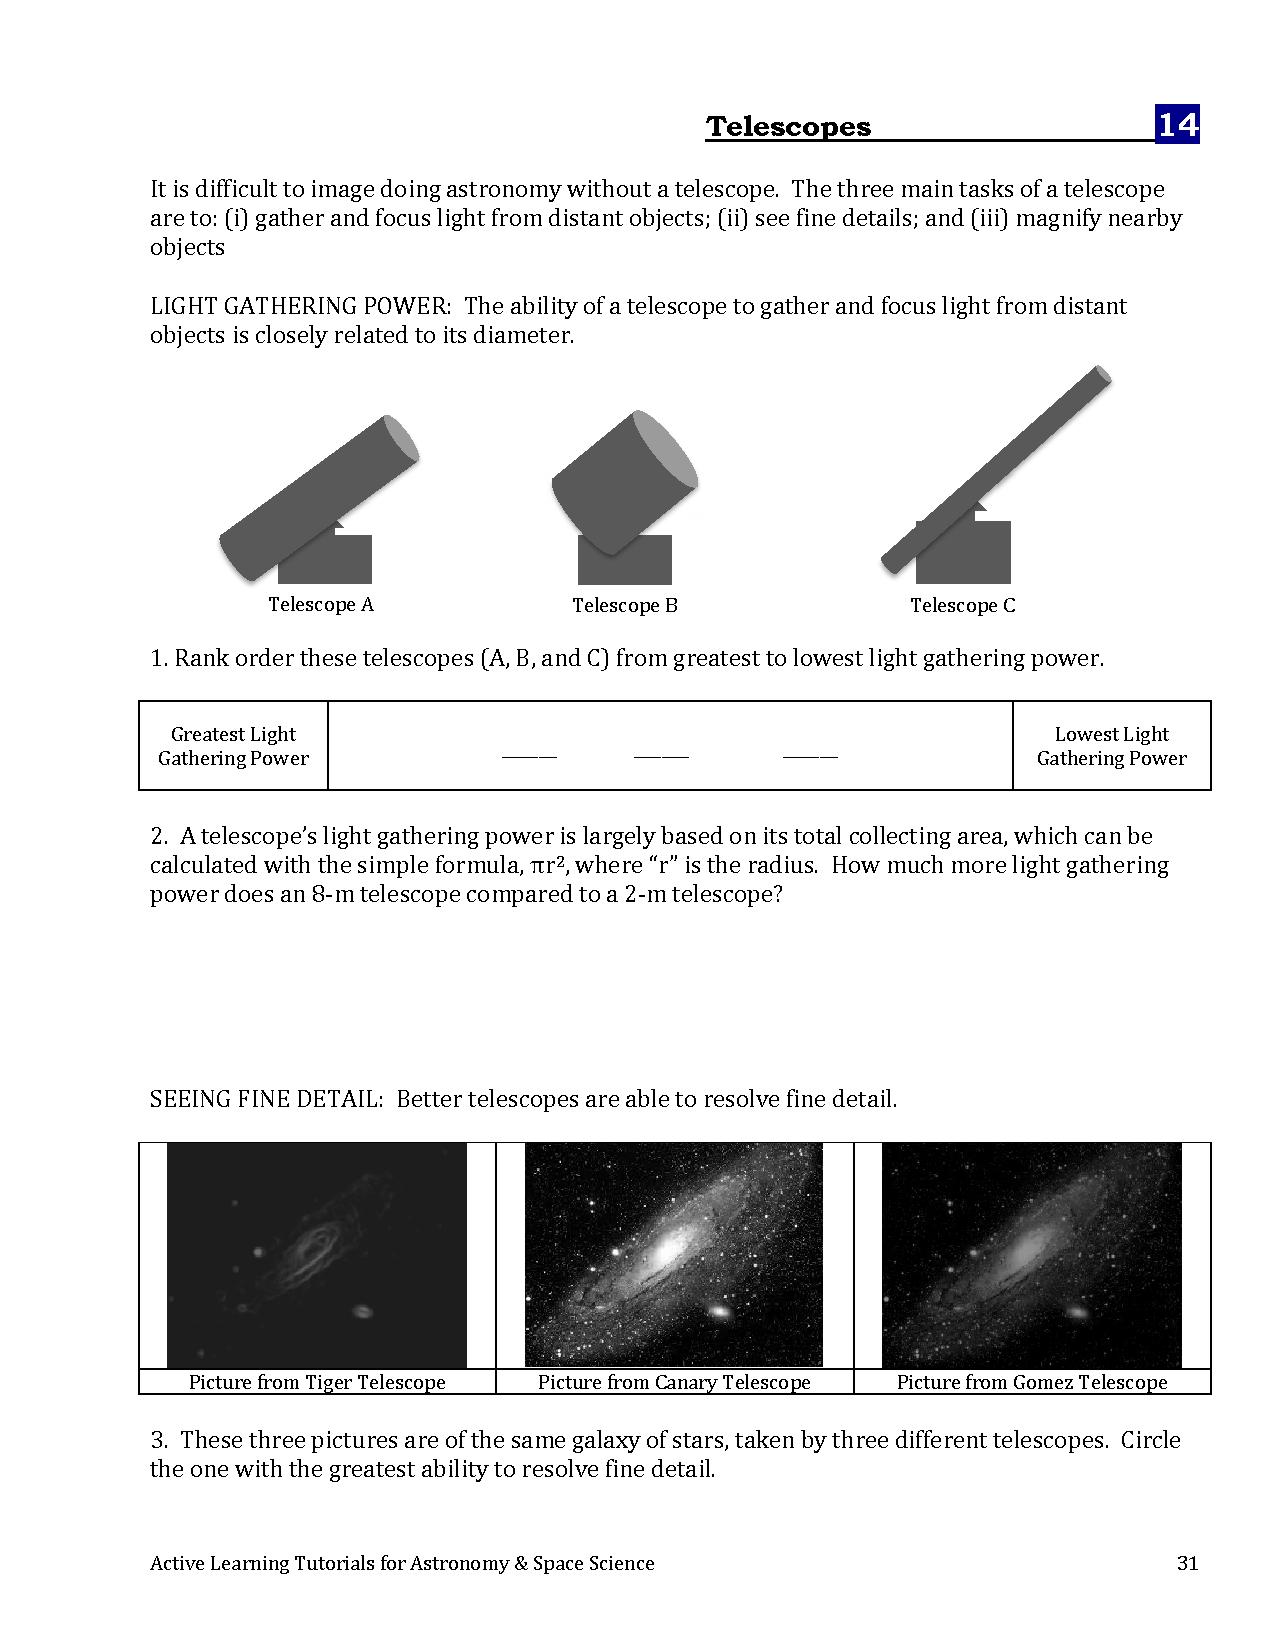
\includepdf[pages={-}]{astro-images-remote/ALT-ASS-Astro-telescopes-angular-res.pdf}

\section{How big is your face?}

This is a simple question, so that you can learn some astronomical concepts and tools while answering it and still keeping the subject matter intuitive.

\subsection{Background: reflecting telescopes and CCDs}

The primary utility of a telescope is its ability to gather light, thereby enabling visualization and analysis of the faint astronomical objects we are trying to observe. This requires focusing light incident on a large surface area. We will be using a \textbf{reflecting} telescope, which means that light rays from observation targets are focused into an eyepiece or onto a detector with reflecting mirrors. This is in contrast to refracting telescopes, which use refracting lenses to focus light rays. Figure~\ref{sot:fig:schmidt} shows schematically how this kind of telescope works. 

\begin{figure}
	\centering
	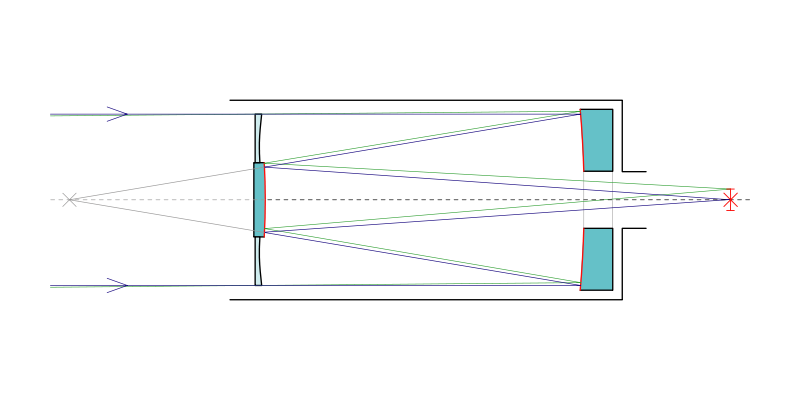
\includegraphics[scale = 0.5]{small-optical-telescopes/Schmidt-Cassegrain-Telescope.png}
	\caption{Schematic for a reflecting telescope of a Schmidt-Cassegrain design. 
		Light rays from astronomical objects enter the telescope in parallel because their source is effectively at infinity. They are then reflected by a parabolic primary mirror onto a secondary mirror that again reflects the light to a focus. An eyepiece or a camera is placed at the focal plane of the resulting image. Image source: \url{https://en.wikipedia.org/wiki/Cassegrain\_reflector\#/media/File:Schmidt-Cassegrain-Telescope.svg}}\label{sot:fig:schmidt}
\end{figure}

%To take images in this lab, and to observe astronomical objects using the SEO, we make use of a \textbf{Charge Coupled Device (CCD)}.
To take images during this lab with your smartphone or digital camera, and for the images taken by the Stone Edge Observatory telescope, we make use of a \textbf{Charge Coupled Device (CCD)}.
CCDs are the standard detectors for taking astronomical images at wavelengths blueward of (lower wavelength than) approximately 1 micron. Think of the observatory's CCD a
very advanced low-noise digital detector, not wholly dissimilar from the digital detector in your
smartphone. Every time a photon within a certain energy range hits the detector, an electron is knocked off of the incident pixel, charging that pixel's capacitor. Thus, for each pixel, more photons $\implies$ more electrons $\implies$ more charge, and the charge can be read off into a digital signal that is then processed as an image. 

%% Don't need to know the following yet, until we play with color.
%The main thing to note is that the CCD material is not sensitive to all wavelengths of light uniformly. Photons of certain energies are more likely to excite electrons in the detector and thus contribute to the output image. Consequently, the observed image intensity will be weighted by the response function of the detector.

\subsection{Finding your pixel scale}

To find out how big your face is the same way you might find out how big a planet is, you need to know the pixel scale of your camera, which is what angle a single pixel covers (this quantity is also your optical system's maximum angular resolution). A simple way is to take an image of something with known angular size, then divide that by the number of pixels it takes up.

\textbf{Equipment:} Smartphone or digital camera, object of known length, ruler or other method of measuring distance across your room, the software SAOImage DS9.

\begin{steps}
	\item Download and install DS9 from \url{http://ds9.si.edu/site/Download.html}. SAOImage DS9, or DS9 for short, is an image viewer, analyzer, and processor written and used by astronomers for working with astronomical images.
	
	If you click the link to download, it might say "redirecting" while never actually redirecting. In this case, copy the link into the address bar directly.
\begin{framed}	
	\textbf{For MacOS}, unless you know otherwise, choose from the top set of choices (to the right of
	the blue apple logo). To find your version, from the Apple menu in the corner of the screen,
	choose “About This Mac”.
	
	If it displays a warning and prevents you from installed from an unidentified developer, follow the instructions at the following link to create an exception:
	
	\url{https://support.apple.com/guide/mac-help/open-a-mac-app-from-an-unidentified-developer-mh40616/mac}
\end{framed}

	\item Set up an object of known length at a known distance from the camera. For example, US Letter sized paper has a standard size, as does currency. You can measure the distance from the camera with a tape measure or other standardized objects. \textbf{Record a length of the object and the distance to the camera, including uncertainty.} Discuss with your group how to estimate the measurement uncertainty.
	
	\item Calculate the angular size of the object and propagate the uncertainty (see Appendix \ref{unc:sec:prop}) from the two measured quantities to report the angular size in the format $A \pm \delta A$.

	To find the angular size of the object, as seen by the camera, you can use the formula
	\begin{equation}
	 \tan \theta = \frac{\textrm{physical size}}{\textrm{distance}}\,.
	\end{equation}
	For situations where the object is far away compared to its size ($\gtrsim 5$ times more distant), you can apply the small-angle approximation, where $\tan \theta \approx \theta$, to simplify the formula to
	\begin{equation}
	 \theta = \frac{\textrm{physical size}}{\textrm{distance}}\,.
	\end{equation}
	Note that the resulting angle will be in radians, not degrees.

\begin{figure}
	\centering
	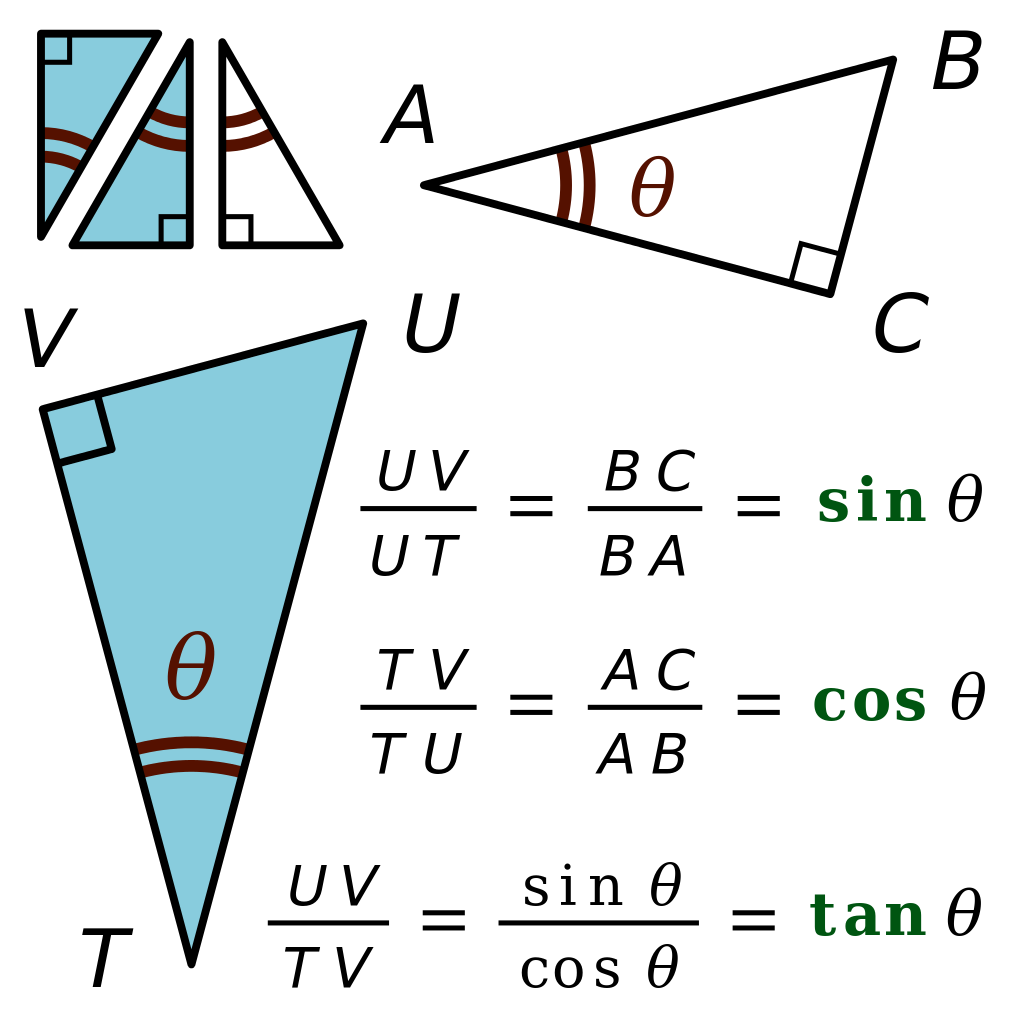
\includegraphics[width=0.35\textwidth]{astro-images-remote/1024px-Academ_Base_of_trigonometry_svg.png}
	\caption{Trigonometric relations for triangles. ``UV'' is the distance between vertices U and V. (Image by \url{https://commons.wikimedia.org/wiki/User:Baelde})}\label{ai:fig:trig}
\end{figure}

	\item Take an image of the object with your camera and copy it to the computer that has DS9 installed on it. \textbf{Include this image in your lab report and label the known object.}
	
	\item The standard image format for astronomical images is FITS. Convert your image to the FITS format at \url{https://www.online-utility.org/image/convert/to/FITS}
	
	\item Open the FITS file in DS9.

\end{steps}
	
	Notice that the image displays in grayscale, and their is another window that opens titled ``Cube'', that has a slider in it. When you move the slider, the image will change slightly. What is happen is that a CCD pixel, by itself, does not know the wavelength of the photon (and thus the color) that it receives. To resolve color, a color filter is placed over the pixel. In consumer cameras, red, green, and blue color filters are attached permanently over different pixels, in a pattern so that all parts of the CCD have equal coverage of the different colors. DS9 reads this and separates the three filters so that each color filter band can be analyzed separately.
	
\begin{steps}
	
	\item Measure the length of the known object in pixels using DS9. There are two ways to do this:
	\begin{enumerate}
		\item One is to place the cursor at each end of the object, record the x and y pixel coordinates at each end, and find the straight-line distance between them (find the x difference and y difference, then use those in Pythagorean's theorem to find the hypotenuse).
		
		\item The other way is to use the ruler tool. To measure a length, select Region $>$ Shape $>$ Ruler from the drop-down menu. Then select Edit $>$ Region. Now if you click and drag on the image, it will draw a line and display the distance in pixels, or in angular separation if the image file has been calibrated withe pixel scale already.
	\end{enumerate}
	
	\textbf{Record the length in pixels and your estimated uncertainty.} To get the uncertainty, you can try doing the above measurement several times and calculate the mean value and the uncertainty of the mean (see Appendix \ref{unc:random}). 
	
	\item Calculate the pixel scale, which is the angular range that each pixel sees. Express it in units of degrees (or arcminutes or arcseconds) per pixel. Find the uncertainty by propagating the uncertainties. \textbf{Record the pixel scale of your camera}.

	\item Based on the pixel scale alone, how far apart in angle would two stars need to be in order to be distinguished as two objects instead of one?

\end{steps}

\subsection{Measuring your face}

Now that you have the pixel scale, you can image another object and find its angular size. And if you know the distance to it, you can find its physical size.

\begin{steps}
	\item Now take a selfie.
	
	\item Use the pixel scale that you determined, along with that image, to find the angular separation between two points in the image --- for example, what is the angle subtended by your eye? Use the distance from the camera to the person to also determine the distance between those two points, for example in millimeters.
	
	\item Estimate the uncertainty, and \textbf{record the angular separation, physical size, and uncertainties for each}.
\end{steps}

%\subsection{Telescope Set Up, Preliminary Observations}\label{ai:sec:setup}
%
%The telescope and camera assembly is an expensive and relatively fragile piece of hardware, so
%move carefully when interacting with the system. We have only two setups, so the class will be split into two groups for using the classroom telescope.
%
%First we will be observing an object at the opposite end of the lab room with the lights turned off. During this exercise we will 1) check that the telescope is focused (which should already be the case), 2) gain practice positioning the telescope and targets, and 3) demonstrate the light gathering and angular resolution capabilities of the telescope with a physical object for which you have an direct sense of scale. \textbf{NOTE: For safety purposes, do not walk around the
%	lab while the lights are off; instead, turn the lights off only as needed to gather data
%	or make observations, and when the lights are off, don’t move about significantly.}
%
%\begin{steps}
%	\item The telescope should already be set up, with the camera on and cooled, and be approximately
%	in focus and pointed at the target at the other end of the lab bench. If not, your TA will
%	work with you to get the setup roughly correct.
%	
%	\item Your first task will be to tweak the centering of the image target. This doesn’t have to be
%	perfect, but you should be able to see the mm scale marks. The telescope can be moved in elevation (up-down). The fine control of elevation is achieved using a knob on the mount - your TA will show you details. To shift the image left or right, move the target instead.
%	
%	\item Next we want to precisely focus the telescope. Do this with most of the lights off --- otherwise
%	the image has too much light. Use the 4th filter of the five available; this can be selected
%	from the ‘Filter’ menu. Then, use the \textbf{Focus} task from the camera control system toolbar,
%	and take images of a few seconds (at most). If the image is completely dark, and the peak intensity number in the focus box is reading around 65000, then the CCD is saturated, and the light in the room should be reduced, or the exposure time shortened.
%	
%	\item Start the focus sequence - the camera will just
%	take and display images repeatedly, of the exposure duration you specified. Now, adjust
%	the focus knob (on the back of the telescope, off center) until you achieve an optimal focus.
%	Note that you can (and should) zoom the magnification of the image so you can see the
%	imaging target in detail. Do this by adjusting the magnification, and adjusting the image
%	x,y centering so you’re looking at an appropriate zoomed location in the image. Note that
%	you’ll need to not be touching the telescope or mount to get a sharp image, so you’ll
%	have to adjust, then move away, wait, and repeat. Your classmates walking around the lab
%	will cause image shake that will make focusing difficult, so enforce a still classroom while
%	you do this.
%
%	\item Once the telescope is focused, \textbf{grab a 1-second exposure} using the Grab command.
%	
%%	\item Time to demonstrate one helpful aspect of telescopes by taking an image in the dark. Once the telescope is focused to the sharpest possible images, turn off the lights and acquire an image using the
%%	\textbf{Grab} button on the toolbar. An exposure time of 40--60 seconds is usually good with all of
%%	the lab lights off and the blinds closed.
%	
%	\item Save this image in ‘fits’ format; the ‘ds9’ tool available on all of the lab
%	computers can be used to examine the image in detail (you can also install this free software on your computer). You can use the university supported
%	’Box’ system to share data with your lab classmates (or any other filesharing app that you prefer). See \url{uchicago.account.box.com/login}
%	for details.
%	
%%	\item With the lights back on, gather around the target on the lab bench and then
%%	turn the light off again. Observe the target. Can you see it? Can you see the details? Does
%%	it matter how close you are (Rubric Row B5)?
%%	
%%	\item Compute and report the ratio of the light gathering power of
%%	the telescope relative to your eye, and comment on how that relates to what you do (or do
%%	not) observe by eye compared to the telescope (Rubric Row B9).
%
%	\item Load the image in DS9. You can adjust the contrast of the image by holding down the right-click and dragging left, right, up, and down. In the upper right window, you can drag the frame around to view different parts of the image. To measure a length, select Region $>$ Shape $>$ Ruler from the drop-down menu. Then select Edit $>$ Region. Now if you click and drag on the image, it will draw a line and display the distance in pixels, or in angular separation if the image file has been calibrated withe pixel scale already.
%	
%	\item In the acquired and saved image you can see a mm scale, which correponds to some number
%	of pixels. Compute and report the ‘pixel scale’ in mm/pixel. Given the distance between the
%	telescope and the target, what is the angular pixel scale in arcseconds/pixel?
%	
%	To find this, note that for an arc (segment) of a circle, the length of that arc $s$ is related to the radius of circle $r$, and the angle (in radians) subtended by that arc $\theta$ by
%	\begin{equation}
%	s = r \theta
%	\end{equation}
%
%	\item Based on the pixel scale alone, how far apart in angle would two stars need to be in order to be distinguished as two objects instead of one?
%	
%	\item Observe the target from the vantage
%	point of the telescope by eye. What detail can you see? How does that compare to what
%	you can see with the telescope?
%	
%	\item Now take an image of part of one of your groupmates with the telescope. Centering on their eye can make for a fun picture. Use the pixel scale that you determined, along with that image, to find the angular separation (or ``angular distance'') between two points in the image --- for example, what is the angle subtended by their eye? Use the distance from the telescope to the person to also determine the distance between those two points, for example in millimeters. %Estimate your uncertainty and compare this measurement to a direct one (by holding up a ruler, for example.)
%\end{steps}

\section{How far apart are these stars?}

Now that you have experience measuring distances for objects you can directly measure, you'll try your hand at measuring distant objects that none of us can measure directly --- stars that were imaged by our robotic telescope at Stone Edge Observatory.
%other stars in your image from SEO!
The goal here is to pick two stars in your image and find the angular separation between them.
%, as well as physical distance. To get the physical distance, you'll need to know their distances from Earth.
To check your work, you can compare to the known positions of these stars. To get that, you'll need to match up those stars in your image to known stars. You can use Stellarium for this, a free virtual observatory app. Then you can select those stars in the app and easily find information about them.

%Note that since we are using a real robotic telescope, many things can go wrong that may result in you not having an image that you've taken. There could have been cloudy nights all week, or smoke from wildfires, or planned power outages to protect from wildfires, or part of the observatory could have broken down. We have archival images in the case that your images are not taken, so that you can still complete the lab.

\begin{steps}
	\item Download the FITS file for 51 Pegasi from the Labs module in Canvas. 51 Peg is the star system where humans detected our first exoplanet.
	
% Second brightest star is Gaia DR2 2832576492727851136. The angular distance between 51 Peg and that one is 0.159841 deg (9'35.4'')
	
	\item Load the image in DS9. You can adjust the contrast of the image by holding down the right-click and dragging left, right, up, and down. In the upper right window, you can drag the frame around to view different parts of the image.

%	\item Log into \url{queue.stoneedgeobservatory.com}, find your completed observation, and click ``go to image''. If you don't have a completed observation, find a classmate's or TA's image URL to visit to get an image to work with. If the image that appears is very fuzzy or has no stars in it, choose a different option from the ``Pipe Step'' drop-down menu.
	
%	\item Select the link ``Download Selected FITS File'' to do so. Open it in DS9.

	\item Also open \url{stellarium-web.org} and search for 51 Pegasi.
	
%	\item Also open Stellarium on a computer. It is a free open source virtual observatory, so you can install it on your computer if you'd like. Use Stellarium to find your target (hover over the left edge of the screen to find the menu that includes the Search function). Toggle the Ground and Atmosphere in the bottom menu, so you can see the star clearly. Zoom in by selecting the rectangle icon third from the right in the upper-right-hand corner. This simulates a field of view that is similar to our telescope.

	\item The field of view (total angular size of image) for SEO is 27', so zoom in Stellarium to the same approximate field of view.
	
	\item Use the Stellarium and the downloaded image to identify two stars, 51 Peg and one other. Note that the two pictures might be rotated or flipped relative to each other.
	
	\item For those two stars, use DS9 to measure the angular separation (angular distance) between them. You may need to use the pixel scale of the Stone Edge Observatory telescope, which is 0.76''/pix (arcseconds per pixel). The image might have "binning" applied, which means that the photons from groups of neighboring pixels were put in the same "bin" (added up), resulting in a larger pixel scale. For example, if the image filename has "bin2" in it, then groups of 2x2 pixels were binned together, so the pixel scale of the image is double the original. \textbf{Record your procedure, value, and uncertainty for the angular separation.}
	
	\item In Stellarium, select each of the two stars in turn and record their equatorial coordinates (RA/Dec). Calculate the angular separation using a web form, for example \url{http://hea.iki.rssi.ru/AZT22/ENG/cgi-bin/c_dist.htm}.
	
	\item Use the $t'$ statistic (see Appendix\ \ref{unc:sec:comparing}) to compare these two values of angular separation.
	
%	\item To find the physical distance between them, use the distances from Earth as given in Stellarium, along with the angular separation and some geometry.
	
%	\item How long does it take light to travel from one of those stars to the other?
\end{steps}

%\section{But wait! Next set of observations with SEO}

%In the next lab, we will be exploring the use of color in astronomical images. The CCD image sensor is monochrome. That is, it has a relatively flat sensitivity to different wavelengths in the visible spectrum. To gain information about color, or the relative contributions of different wavelengths, you'll use filters that can be placed in front of the sensor. So for next week, \textbf{queue another observation or several} (no more than 1 per student per week). Choose the same target from last week. Select the r, g, and b filters (red, green, and blue, respectively), and leave the "dark" checked as well. For the exposure time, you can adjust it if you think the image was over- or under-exposed, but be careful --- the color filters cut down the intensity of light, even in the color that it transmits the most, by at least a factor of two.

\section{Report checklist and grading}

Each item below is worth 10 points. See Appendix\ \ref{cha:lab-report-format} for guidance on writing the report and formatting tables and graphs.

\begin{enumerate}
	
	\item Completed telescopes and angular size worksheets.
	
	\item Image of the known object, with object labeled, along with measurements and calculations for the angular size of the known object, with uncertainties (Steps 3--4)
	
	\item Length calculated with DS9, with the calculation of pixel scale and its uncertainty (Steps 7--8)
	
	\item Image of selfie, calculation of angular separation, physical size, and uncertainties (Steps 10--12)
	
	\item Image from SEO, with your two stars marked, along with the calculation of angular separation. (Step 18)
	
	\item Calculation of angular separation from Stellarium's coordinates, along with the comparison using the $t'$ statistic (Steps 19--20)
	
	\item Discuss the findings and reflect deeply on the quality and importance of the findings. This can
	be both in the frame of a scientist conducting the experiment (“What did the experiment tell us
	about the world?”) and in the frame of a student (“What skills or mindsets did I learn?”).
	
	\item A 100–200 word reflection on group dynamics and feedback on the lab manual. Address the
	following topics: who did what in the lab, how did you work together, what successes and
	challenges in group functioning did you have, and what would you keep and change about the
	lab write-up?
	
	\item Write a paragraph reporting back from each of the four roles: facilitator, scribe, technician,
	skeptic. Where did you see each function happening during this lab, and where did you see
	gaps?
\end{enumerate}
\chapter{Inventing Color}

Everything glows (gives off electromagnetic radiation) when it has a temperature --- particles are wiggling around randomly (faster if it's hotter) and giving off energy as they wiggle. This \textbf{thermal radiation}, also called blackbody radiation, is the same for any object at the same temperature. This means we can take something's temperature by looking at the spectrum of light it gives off. This is great for learning about something's temperature at a distance, like stars.

Incandescent lightbulbs are so warm that they glow in the visible spectrum (like stars). In this lab, you'll investigate the radiation that is given off by a lightbulb at various temperatures, then use filters to mimic the situation astronomers are in when they observe astronomical objects with different color filters. You'll invent a metric to numerically state the temperature of the lightbulb, even without knowing the actual temperature. Finally, you'll use the various images that you took with SEO with different color filters and combine them to form a color image.

\section{Lightbulbs}

\begin{steps}
	\item Using the spectrometer, observe the spectrum created by a lightbulb at various brightnesses / voltages.  What's the overall shape? How does the shape change when the brightness increases? How does the peak frequency change? How does the visual color of the bulb change as it gets brighter? As the lightbulb gets brighter, the filament inside gets hotter. If all objects act like the tungsten filament as it gets hotter, what general pattern can you state about the EM radiation given off by an object as a function of its temperature?

\end{steps}

Cameras have come a long way since the days of developing film, but sensors are not as smart you might think. They register light, but they can't usually tell the color (i.e. wavelength) of the incoming photons. So then how do you get a color image? In astronomy (and in your cell phone!) color images are generated by measuring the amount of light at specific colors and then combining these measurements to create a colorful image. A filter is used to select bands of color to allow through. In consumer cameras and phone cameras, these filters are permanently attached to the front of individual pixels. In astronomical imaging, there is no permanent filter, and different filters are moved into place.

\begin{steps}
	\item Use the red and green filters in front of the fiber optic input to the spectrometer to see how they affect the spectrum that is received. \textbf{Save a graph of the spectrum with each filter and include in your report.}
\end{steps}

In a regular astronomical image, each pixel gives just one value --- the number of counts detected in that pixel, regardless of the wavelength of the photon detected. We can treat the fiber optic as a single-pixel camera if we count up the total number of counts detected. To find that total number, you can find the area under the curve in the plot.

\begin{steps}
	\item With no filter, add up the total number of counts detected by calculating the area under the curve. To do this in an approximate way, count the number of boxes underneath the curve, then multiply this by the height of one box (in counts per nanometer) and by the width of one box (in nanometers).
	
	\item Do the same for the spectrum using the red and green filters separately.
\end{steps}

Now you have the value of our single-pixel camera for the case of clear (no filter), red, and green filters. Time to revisit the pattern found above in Step 1.

\begin{steps}
	\item If that pattern from Step 1 is true, what should happen to the relative values of red and green as the voltage is increased? Should one increase more than the other?
	
	\item Perform an experiment to test whether this prediction is supported.
\end{steps}

\section{Creating a color image}

Now you'll create a color image from the three images you took last week, of the same target with r, g, and b filters.

\textbf{Loading and manipulating images in ds9 consists of:}
\begin{itemize}
\item loading an image  (file > open)
\item setting z1,z2 on an image  (scale > various algorithms; use scale > scale parameters for full control). See Figures \ref{ic:fig:z-min-max}--\ref{ic:fig:z-small} for examples.
\item controlling the intensity mapping within those bounds (mouse right click-and-hold and drag)
\end{itemize}

\begin{figure}
	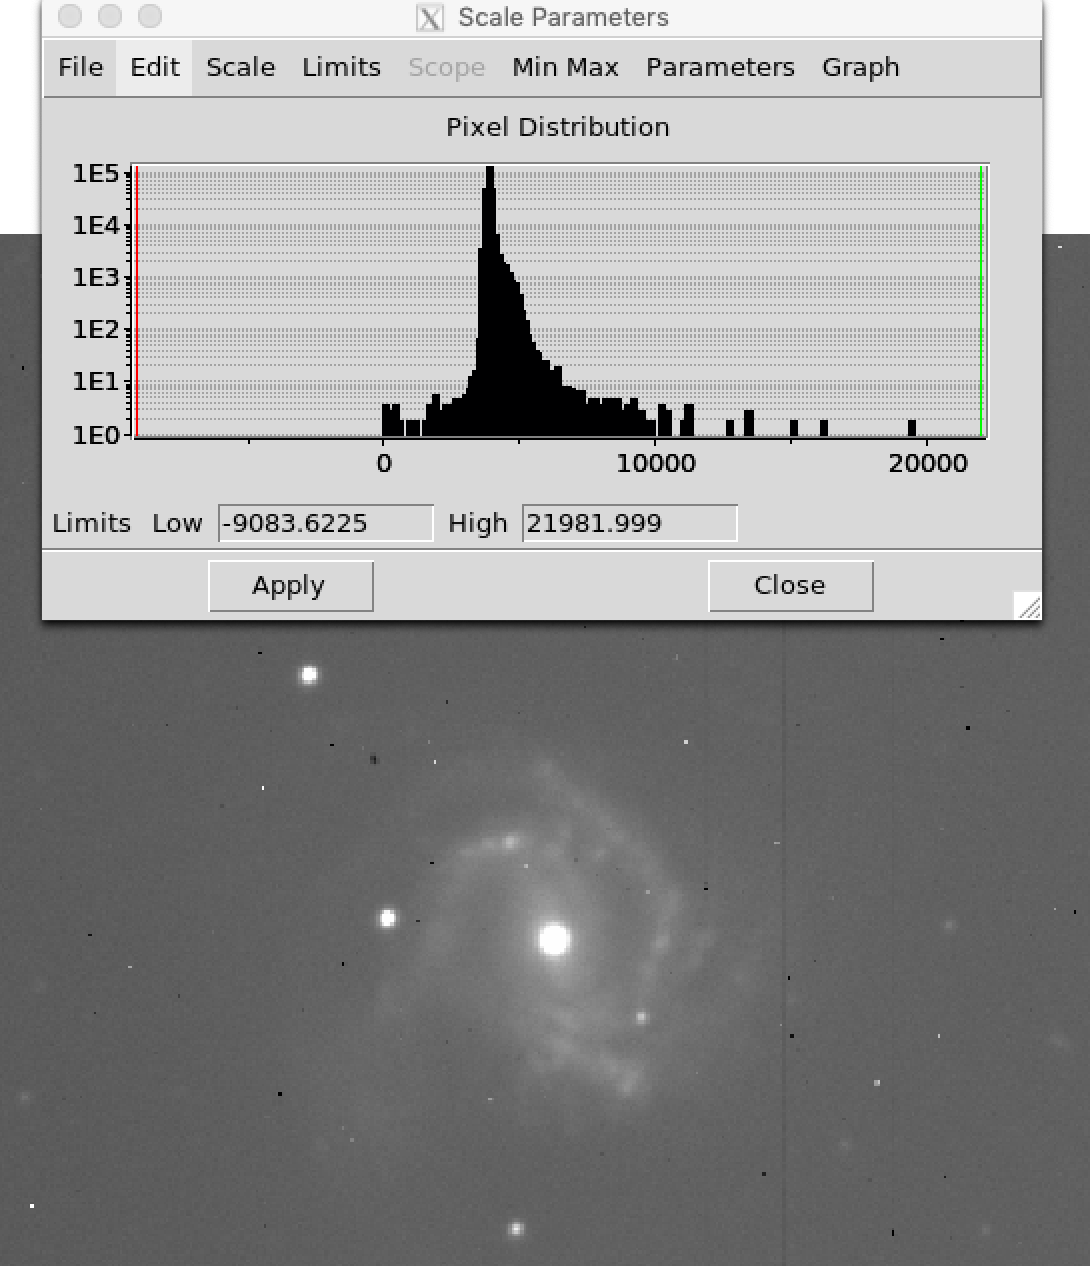
\includegraphics[width=0.5\textwidth]{inventing-color/z-min-max}
	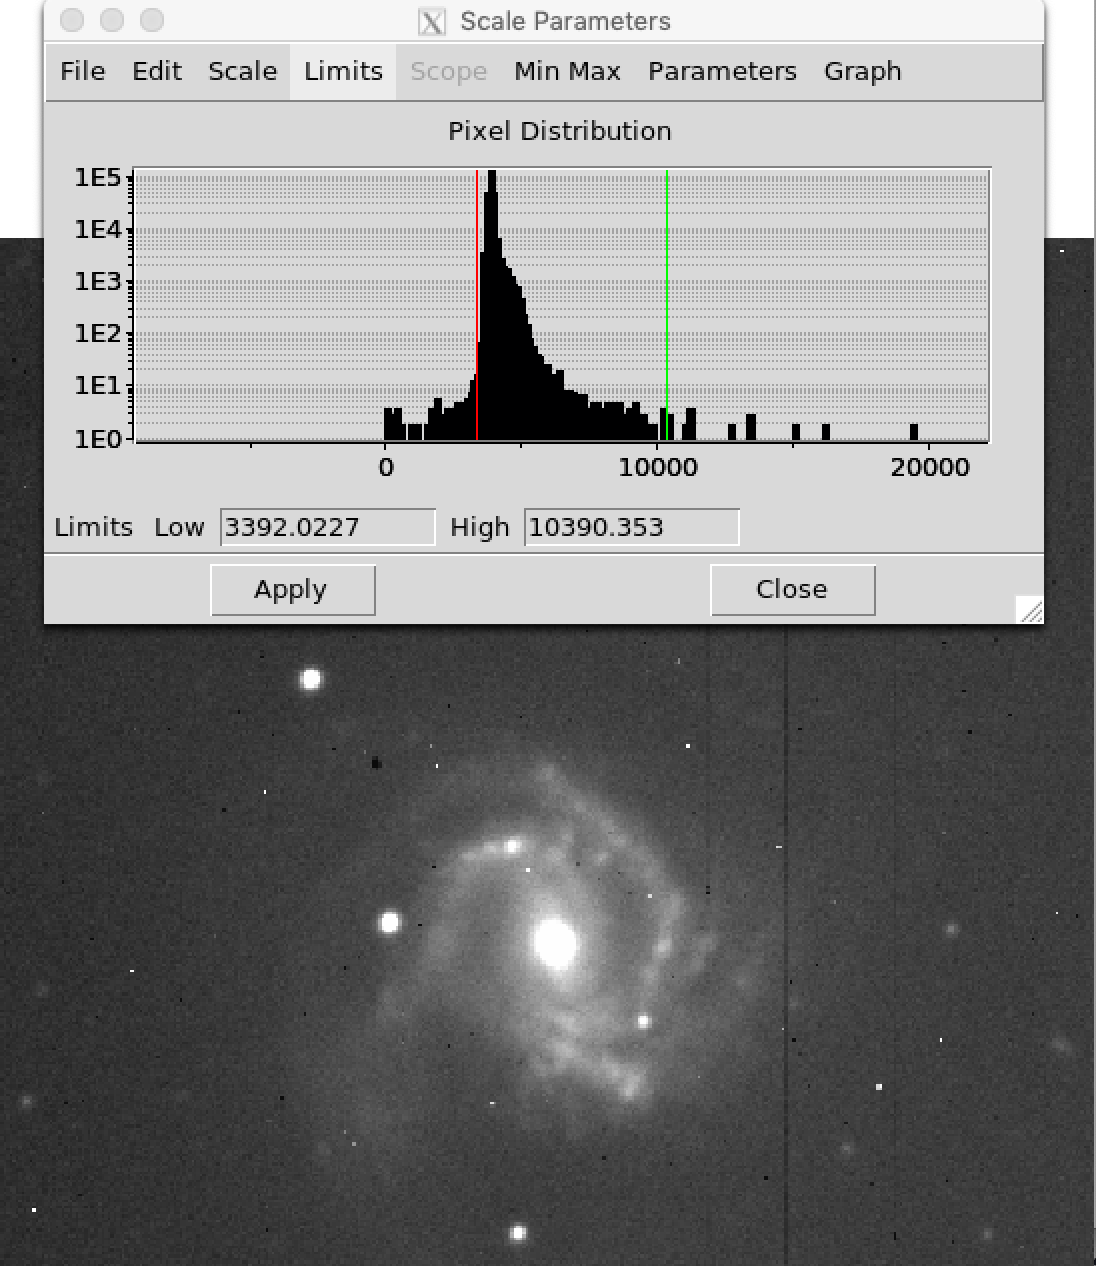
\includegraphics[width=0.5\textwidth]{inventing-color/z-mid}
	\caption{Proper choice of data ranges is important. The default for ds9 is often the min/max values in the image, which can be a poor choice if there are outlier pixels, as shown here on the left. The red line shows the lower limit z1, which is mapped to no color (black here), and the green line is the upper limit z2, mapped to full color (white here). Pixel values between these are shown in various brightnesses of the color. On the right, z1 and z2 are more tuned to the distribution of pixel values, which more effectively uses the dynamic range of the display for pixel values where there are significant amounts of data.}\label{ic:fig:z-min-max}
\end{figure}

\begin{figure}
		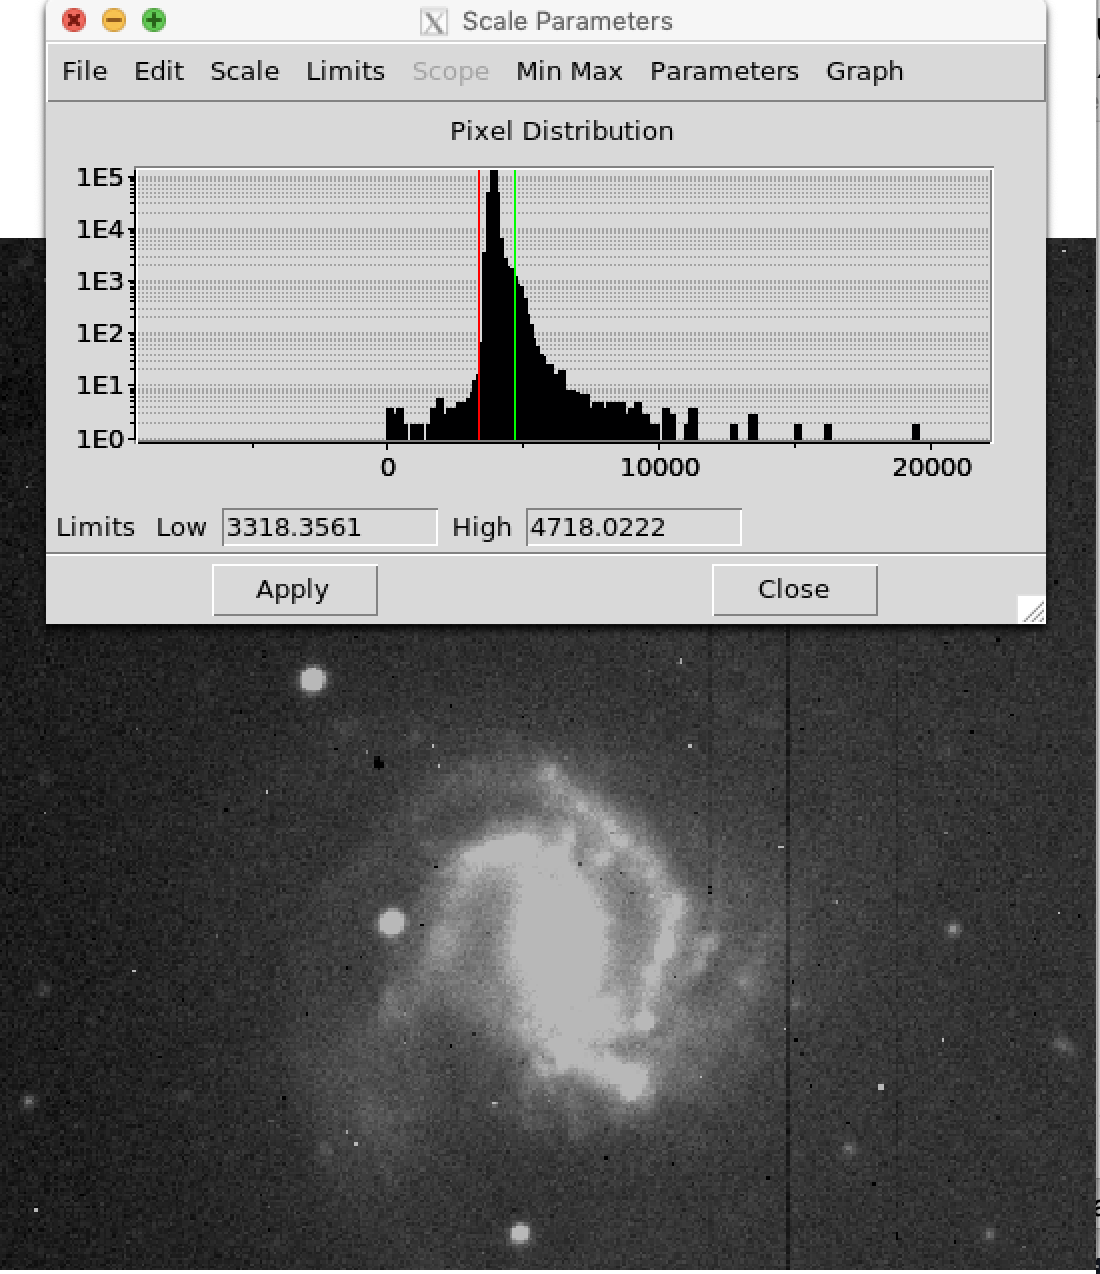
\includegraphics[width=0.5\textwidth]{inventing-color/z-small}
		\caption{Smaller values of z2 will emphasize fainter values in the target. Compare the image to the left to the right-hand image above.}\label{ic:fig:z-small}
\end{figure}

\textbf{You can change the zoom and center location in an image by} 
\begin{itemize}
\item moving around in image (mouse middle click if edit>point is set[the default], or edit>pan and mouse left click)
\item zooming in and out (mouse wheel, zoom> +,- etc.)
\end{itemize}

\textbf{To build a color image}
\begin{itemize}
\item Open a color (rather than monochrome) frame:  Frame > new rgb
\item Open the red, green, blue files using the rgb subwindow to select which channel you are working in, and then scale and control intensities on each one. 
\item There are many possible ways to scale the images. Some testing suggests that choosing Scale > ASINH (or Linear or Square Root as other choices) and Scale > 99.5\% (or maybe 99\% or 98\%)  produces reasonable results. Experiment!
\item One thing to note: the rgb subwindow allows you to control how the images are aligned spatially via the “align” menu at the top. There are three relevant choices: “WCS”, “Image” or “Physical”.  The latter two should give the same result in this instance. “WCS” alignment uses information in the image header that has been added by the processing pipeline, that establishes a World Coordinate System (this tells ds9 and other programs how pixel x,y values are mapped into the sky coordinates - typically Right Ascension [east/west] and Declination [north/south]). The default is WCS and should work fine, if the images processed correctly. If that doesn’t look good, you could try the others. If that still doesn’t look good, note that you tried your best, and give an example of how it didn’t work will in either mode. Examples of good and bad image alignment are shown in Figure \ref{ic:fig:rgb-bad}.
\end{itemize}

\begin{figure}
	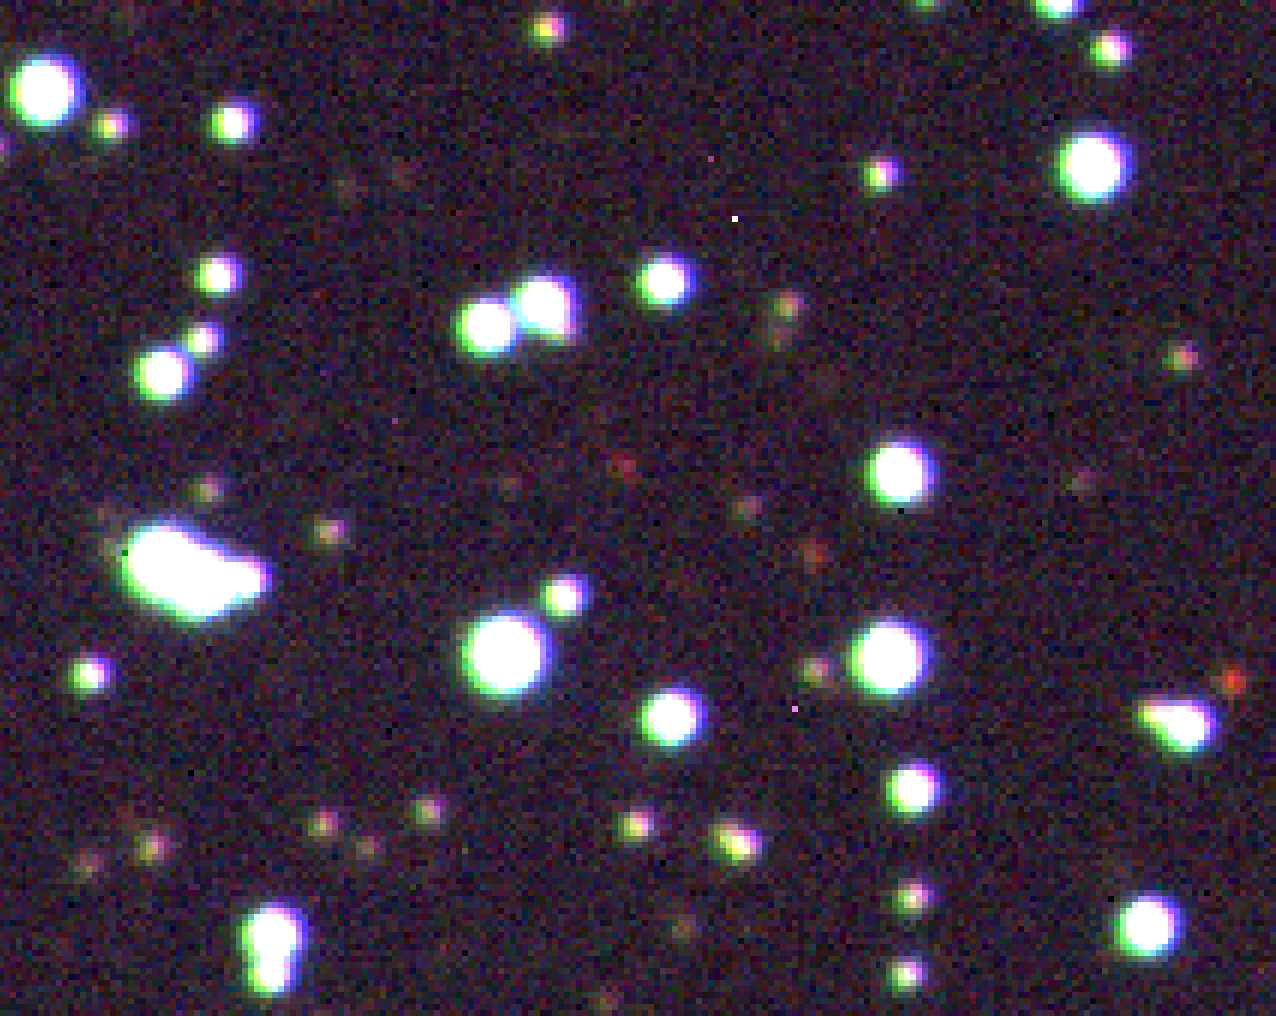
\includegraphics[width=0.5\textwidth]{inventing-color/rgb-bad}
	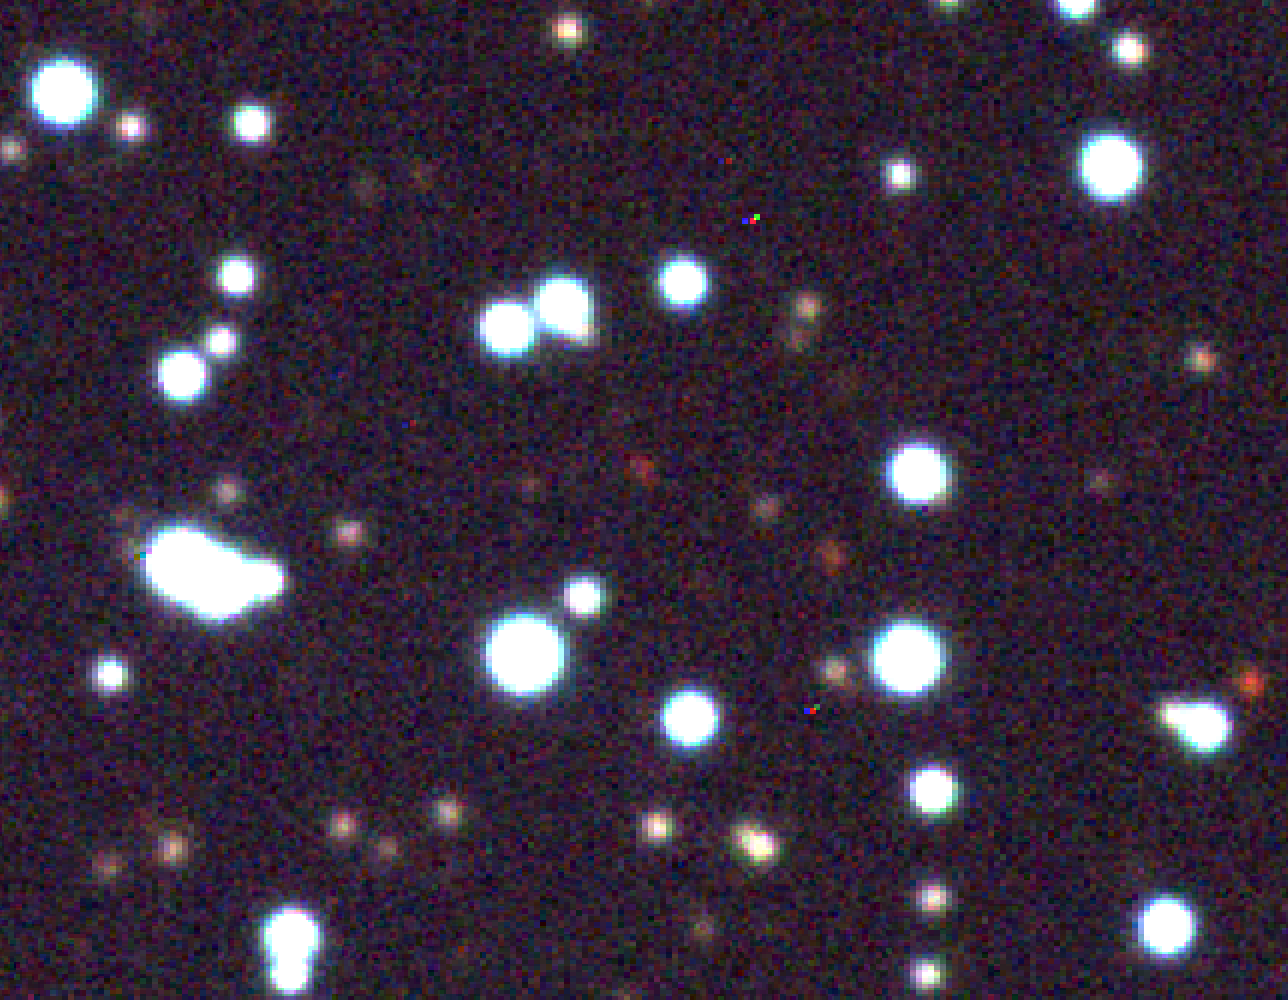
\includegraphics[width=0.5\textwidth]{inventing-color/rgb-good}
	\caption{Zoom-in on a color image, showing poor (left) and good (right) image alignment across filters. Note how objects are shifted between different color channels in the poorly aligned image.}\label{ic:fig:rgb-bad}
\end{figure}
%\chapter{The HR-Diagram}

\section{Introduction}

In this lab we will analyze our observations of star clusters to make one of the key figures in all of observational astronomy - the Hertzsprung-Russell (HR) Diagram. This will give us insight into the stellar populations in the clusters we observe, and allow for an estimate of the cluster ages. 

\section{Learning goals}

\begin{itemize}
    \item Gain an understanding of astronomical image analysis and photometry
	\item Gain practice performing basic calculations on datasets and making informative scientific figures from those data
	\item Learn where different stellar populations lie on the HR diagram, and understand the physical reasons behind these localizations
	\item Estimate stellar cluster ages using the predictions of stellar evolutionary models. 
\end{itemize}

\section{Scientific background}

Stars evolve (i.e., change their properties) over millions and often billions of years – too slow for us to see the evolution over a human lifespan.  Such impressive longevity is due to the fact that stars are powered by thermonuclear reactions, which are very efficient in generating abundant energy and have quite a bit of fuel to last for a long time. Stars like our Sun last about 10 billion years (so the Sun is in its middle age). The long timescale of evolution also means that we have to develop a different way to study stellar evolution. 

Astronomers explore evolution of stars by observing large populations of stars where different stars are in different stages of evolution. Of course, in order to do this we need to be able to tell which star is in what stage. This is done by a combination of observations – which measure luminosity and surface temperatures – and theoretical models – which predict how luminosity and surface temperature change as stars evolve. The key is that luminosity and temperature at a certain age are determined by star's mass, chemical composition, and details of thermonuclear reactions (which elements are burning, over what fraction of star's volume, etc.).

Luminosity and temperature of stars are related because they are both determined by their internal structure, which, in turn, is determined by the basic physical properties (mass, chemical composition, age). Therefore, stars are not scattered randomly in the luminosity and temperature space but follow well-defined sequences, which reflect the ranges of the controlling parameters in a given stellar population. 

The surface temperatures of stars can be deduced by fitting a blackbody radiation spectrum to their spectra. Even for stars that do not have spectra measured, their temperatures can be deduced from their colors (Recall: does bluer color correspond to cooler or hotter temperature?). Our eyes and brain perceive color by analyzing spectral composition of the incoming light. In astronomy, a star's color is defined as the difference between its magnitudes measured through two different filters that block out all light except light within a fairly narrow range of wavelengths. 

In order to interpret evolutionary states, we look at physical groupings of stars called stellar clusters, which are located at the same distance from us and were born at the same time from the same cloud of dense gas. The spread in their properties will thus not be due to different ages or initial compositions, but mainly due to different masses. As you will see, stars occupy distinct regions of the observable equivalent of the luminosity-temperature space – the magnitude-color space called the Hertzsprung-Russell (HR) diagram. We will make this diagram for the star cluster we observed.

\section{Obtaining Images}

To view images taken by the SEO and download the associated data, sign into your account on the queue website (\texttt{https://queue.stoneedgeobservatory.com/}), navigate to \texttt{OBSERVATIONS} $\blacktriangleright$ \texttt{MY OBSERVATIONS}. The observation you queued should be listed, and \texttt{Yes} should appear in the \texttt{Completed} column if the data have been taken. To view and download completed observations, click \texttt{Actions} $\blacktriangleright$ \texttt{Go To Images}. This will link you to an external page with both an image viewer and links(?) to directly download the data. This can be accomplished with the \texttt{Download Selected FITS File}. Make sure that the \texttt{Pipe Step} option under \texttt{Selection} is listed as \texttt{FludxCalibrated}, since this is the reduced and calibrated data. There are other data products from both the observation and data reduction process available from this page, but we aren't using them for our analysis. Unfortunately, the data reduction process does not work on every observation, so if one or both of your observations lacks \texttt{FluxCalibrated} option, share data with a group that does.\textit{Note that you cannot use data from different observations for both filters - i.e. observations from both filters analyzed by each group need to be of the same exposure time}. Download these data onto your local machine where you will perform your analysis.

\section{Analyzing the data in DS9}

To analyze our observations we will be using DS9 (\texttt{http://ds9.si.edu/site/Home.html}), a popular software package for the visualization and basic analysis of image data within the astronomical community. If you are working on a lab computer, the software is already installed. If you are using your personal computer, it can be downloaded and installed from the provided link. 

We will use this tool to measure the flux in both observed filters for as many stars as possible. Each group should use separate, adjacent computers - bring up images in DS9 for each filter, one filter per computer. To better visualize the images in DS9, logarithmically scale the display by selecting \texttt{scale} $\blacktriangleright$ \texttt{log}. Contrast and bias of the display image can be modified by clicking and dragging - you should adjust these so that the stars are optimally visible.

To determine how much flux comes form each star, we will use the ``regions" functionality of DS9 that gives information about a selected region in the image. First click \texttt{edit} $\blacktriangleright$ \texttt{region}, and then you will create a region -- indicated by a green circle -- each time you click on the image. Clicking in the center of the region will allow you to move it about the image, while clicking on the edge allows you to adjust it's size. For each star you measure, you'll want to create a region that contains as much flux as possible without contamination from a nearby star or the background. Once this is accomplished, double click the region (which will cause a window with basic information to appear), and select \texttt{Analysis} $\blacktriangleright$ \texttt{Statistics}, which will cause a separate panel to appear with information about the data contained in that region. ``Sum" is the flux (in an astronomy-specific unit called ``Janskys", abbreviated as Jy) value you should record. Also recod the ``Center" coordinates and radius of the region. Do this in both filters, for each star that you measure. \textit{Note that the error listed under ``Statistics" is \textbf{not} a correct estimate of the error in the flux value, so do not record this}.

Error in your measurement can be the result of several causes, but one that is easy to quantify is the presence of background noise (from e.g. sky brightness or scattered light in the telescope). From several circular regions over nothing in particular, determine how many counts there are per unit area, just from the backgrounds.  The “surf$\_$bri” value gives what we need.  Do this several times to determine the variance in the background, and also how it varies over the different parts of the image.  Thus quantify this background and its error. For each of your stars, compute the background that was likely in the aperture.  This involves multiplying the surface brightness by the area you chose.  The error in the surface brightness propagates, so if you have a very big region, that will likely determine the error on your final measurement. 

Try to measure fluxes and errors for as many stars as possible in your lab session. There will inevitably be some overlap between groups, which is fine, but try to obtain measurements for stars at a wide range of brightness’s. 50 stars is a good target, but the more the better. Thirty minutes before lab ends, stop collecting data, and share your data among your section so that you can finish the rest of the analysis.

\section{Calculating Magnitudes}

In astronomy we deal with magnitudes, which are scaled logarithmically, and increase with decreasing source brightness. Specifically, the equation for the magnitude $m_X$ of an object in a wavelength band $X$ with flux $F_X$ is given by 

\begin{equation}
m_{X} = -2.5\log_{10}\left(\frac{F_X}{F_{X,{\textrm{ref}}}}\right)
\end{equation}

where $F_{X,{\textrm{ref}}}$ is a reference flux value for the given band and magnitude system. For the SDSS magnitude system we are using, $F_{\textrm{ref}} = 3631 {\textrm{Jy}}$ for both $g'$ and $r'$ measurements. Calculate magnitudes in both bands for all of the stars measured in your section. You can use Excel or any other software/coding language of your choice to do this.  

\section{Making an HR Diagram}

Since different bands measure brightness in different wavelengths, the ratio of flux in two bands is a measure of an object's color. Therefore, the difference between astronomical magnitudes of an object in different bands is a measure of its color, since the magnitude scale is logarithmic:

\begin{equation}
m_A - m_B = -2.5\log\left(\frac{F_A}{F_B}\right).
\end{equation}

An H-R diagram is a plot of stellar magnitude vs. color - aka a ``color magnitude diagram''. A star's color is an observational indication of it's surface temperature. Since all of the stars in a star cluster are at approximately the same distance, their apparent magnitude gives a good relative indicator of luminosity. Therefore, a color-magnitude diagram of stars at roughly constant distance is effectively a temperature-luminosity diagram, and stars fall in characteristic regions of this parameter space based on their mass, age, and metallicity.

We have data in two wavelength bands, so we can subtract those magnitudes to get a color measure. With the software or coding language of your choice, plot $r'$ on the y-axis and $g' - r'$ on the x-axis. Add error bars to your plot. If this becomes crowded on your figure, you can estimate a typical error from your data and include it in a legend. 

\section{Making an HR Diagram -- with proper photometry}

In reality, your estimated error from the background is a lower limit, since there are many other possible sources of imprecision and innacuracy in this measurement. Moreover, our analysis was an extremely crude approximation of the photometry done by professional astronomers. To make HR diagrams that can be interpreted scientifically, use the data provided for the cluster you observed, each of which has a .csv file [provided on the lab computer? the course website?]. Note that, if you observed NGC 869, the publicly available data was made with different fileters than our observations, and thus the expected positions of stellar populations on a color-magnitude diagram change, but the same general features shold be apparent. Label the differet stages of stellar evolution on both the professionally reduced data and, if possible, on the data you obtained in lab.   

\section{Comparing to stellar evolution models}

The last portion of this lab involves estimating the age of these stellar populations by comparing their color magnitude diagrams with predictions from a stellar evolution model. Stellar physics is sufficiently well-understood that accurate evolutionary models have been constructed to calculate the observable properties of stars across their lifetimes. Because stars evolve in their position on the HR diagram, we can estimate the age of our observed cluster by comparing these models to our observations.

Several files containing model predictions for the magnitudes of stars at different ages are contained in files that will be provided to you. These have been calculated using the observed metallicity of the star cluster to predict the positions of stars at ages $10^7$, $10^8$, $10^9$, and $10^{10}$ years. These are called isochrones - stellar properties as a function of stellar mass for a fixed age. Note that these magnitudes have been corrected for cluster distance and extinction due to intervening galactic dust.

Plot these isochrones on your HR diagrams and compare them to your data to estimate the cluster age. What physical changes in stellar properties are represented by the different locations of isochrones of different ages? What physical processes in the star underlie those properties?



%\chapter{Self-Directed Experiment}

You've spent the last 4 weeks learning various techniques for collecting and analyzing astronomical data. Now it's your turn to choose a project and use those techniques more independently to answer a scientific question that you choose. At least, you can choose from a list, so it is more likely you'll find a project that appeals to you.

So in the next two weeks, you will conduct the experiment / project, and in the following week, you will present your findings in class (as well as submitting a written report). Our goal is for you to work more independently than in past weeks, and also use your TA, professor, and teaching support manager for assistance when needed.

\section{Project A: Use of different wavelengths to see different things}

\section{Project B: When did the Crab Nebula star explode?}

\section{Project C: How heavy is the binary star system 61 Cygni AB?}

\section{Project D: How hot is the Sun?}

\section{Project E: How fast are stars moving and why?}

\section{Project F: Thin/thick disk populations?}

\appendix

\chapter{Analysis of Uncertainty}

A physical quantity consists of a value, unit, and uncertainty.
For example, ``$5 \pm 1\,$m'' means that the writer believes the true value of the quantity to most likely lie within 4 and 6 meters\footnote{The phrase ``most likely'' can mean different things depending on who is writing.
	If a physicist gives the value and does not given a further explanation, we can assume that they mean that the measurements are randomly distributed according to a normal distribution around the value given, with a standard deviation of the uncertainty given.
	So if one were to make the same measurement again, the author believes it has a 68\% chance of falling within the range given.
	Disciplines other than physics may intend the uncertainty to be 2 standard deviations.}.
Without knowing the uncertainty of a value, the quantity is next to useless.
For example, in our daily lives, we use an implied uncertainty.
If I say that we should meet at around 5:00 pm, and I arrive at 5:05 pm, you will probably consider that within the range that you would expect.
Perhaps your implied uncertainty is plus or minus 15 minutes.
On the other hand, if I said that we would meet at 5:07 pm, then if I arrive at 5:10 pm, you might be confused, since the implied uncertainty of that time value is more like 1 minute.

Scientists use the mathematics of probability and statistics, along with some intuition, to be precise and clear when talking about uncertainty, and it is vital to understand and report the uncertainty of quantitative results that we present.

\section{Types of measurement uncertainty}

For simplicity, we limit ourselves to the consideration of two types of uncertainty in this lab course, instrumental and random uncertainty.

\subsection{Instrumental uncertainties}

Every measuring instrument has an inherent uncertainty that is determined by the precision	
  of the instrument.
Usually this value is taken as a half of the smallest increment of the instrument's scale. For example, $0.5\:$mm is the precision of a standard metric ruler; $0.5\:$s is the precision of a watch, etc. For electronic digital displays, the equipment's manual often gives the instrument's resolution, which may be larger than that given by the rule above.

Instrumental uncertainties are the easiest ones to estimate, but they are not the only source of the uncertainty in your measured value.
You must be a skillful experimentalist to get rid of all other sources of uncertainty so that all that is left is instrumental uncertainty.

\subsection{Random uncertainties}

Very often when you measure the same physical quantity multiple times, you can get different results each time you measure it.
That happens because different uncontrollable factors affect your results randomly.
This type of uncertainty, random uncertainty, can be estimated only by repeating the same measurement several times.
For example if you measure the distance from a cannon to the place where the fired cannonball hits the ground, you could get different distances every time you repeat the same experiment.	
  
For example, say you took three measurements and obtained 55.7, 49.0, 52.5, 42.4, and 60.2 meters. We can quantify the variation in these measurements by finding their standard deviation using a calculator, spreadsheet, or the formula (assuming the data distributed according to a normal distribution)
\begin{equation}
 \sigma = \sqrt{\sum_{i=1}^{N} \frac{(x_i-\bar{x})^2}{N-1}} \, ,
\end{equation}
where $\{x_1, x_2, \dots, x_N\}$ are the measured values, $\bar{x}$ is the mean of those values, and $N$ is the number of measurements.
For our example, the resulting standard deviation is 6.8 meters. Generally we are interested not in the variation of the measurements themselves, but how uncertain we are of the average of the measurements. The uncertainty of this mean value is given, for a normal distribution, by the so-called ``standard deviation of the mean'', which can be found by dividing the standard deviation by the square root of the number of measurements,
\begin{equation}
\sigma_\textrm{mean} = \frac{\sigma}{\sqrt{N}} \, .
\end{equation}
So, in this example, the uncertainty of the mean is 3.0 meters. We can thus report the length as $52 \pm 3\:$m.

Note that if we take more measurements, the standard deviation of those measurements will not generally change, since the variability of our measurements shouldn't change over time. However, the standard deviation of the mean, and thus the uncertainty, will decrease.

\section{Propagation of uncertainty}

When we use an uncertain quantity in a calculation, the result is also uncertain. To determine by how much, we give some simple rules for basic calculations, and then a more general rule for use with any calculation which requires knowledge of calculus. Note that these rules are strictly valid only for values that are normally distributed, though for the purpose of this course, we will use these formulas regardless of the underlying distributions, unless otherwise stated, for simplicity.

If the measurements are completely independent of each other, then for quantities $a \pm \delta a$ and $b \pm \delta b$, we can use the following formulas:
\begin{equation}\label{unc:add}
\textrm{For } c = a + b \textrm{ (or for subtraction), } \delta c = \sqrt{(\delta a)^2 + (\delta b)^2}
\end{equation}

\begin{equation}\label{unc:mult}
\textrm{For } c = ab \textrm{ (or for division), } \frac{\delta c}{c} = \sqrt{\left(\frac{\delta a}{a}\right)^2 + \left(\frac{\delta b}{b}\right)^2}
\end{equation}

\begin{equation}\label{unc:exp}
\textrm{For } c = a^n,\, \frac{\delta c}{c} = n \frac{\delta a}{a}
\end{equation}

If you are familiar with calculus, you may want to use this general formula for the uncertainty $\delta f$ of a function $f$ of $N$ independent values $x_i$, each with uncertainty $\delta x_i$:
\begin{equation}\label{unc:general}
\delta f = \sqrt{ \sum_{i=1}^{N} \left(\frac{\partial f}{\partial x_i} \delta x_i\right)^2 } \, .
\end{equation}
Notice that Eqs.\ \ref{unc:add} through \ref{unc:exp} can be derived from Eq.\ \ref{unc:general} for those specific cases.

\subsubsection{What if there is no reported uncertainty?}

Sometimes you'll be calculating with numbers that have no uncertainty given.
In some cases, the number is exact.
For example, the circumference $C$ of a circle is given by $C = 2 \pi r$. Here, the coefficient, $2\pi$, is an exact quantity and you can treat its uncertainty as zero.
If you find a value that you think is uncertain, but the uncertainty is not given, a good rule of thumb is to assume that the uncertainty is half the right-most significant digit.
So if you are given a measured length of $1400\:$m, then you might assume that the uncertainty is $50\:$m.
This is an assumption, however, and should be described as such in your lab report.
For more examples, see Table~\ref{unc:tab:implied}.

\begin{table}
	\begin{center}
		\begin{tabular}{cc}
			\textbf{Expression} & \textbf{Implied uncertainty} \\
			12 & 0.5 \\
			12.0 & 0.05 \\
			120 & 5 \\
			120. & 0.5
		\end{tabular}
		\caption{Expression of numbers and their implied uncertainty.}\label{unc:tab:implied}
	\end{center}
\end{table}

\subsubsection{How many digits to report?}

After even a single calculation, a calculator will often give ten or more digits in an answer.
For example, if I travel $11.3 \pm 0.1\:$km in $350 \pm 10\:$s, then my average speed will be the distance divided by the duration. Entering this into my calculator, I get the resulting value ``\texttt{0.0322857142857143}''.
Perhaps it is obvious that my distance and duration measurements were not precise enough for all of those digits to be useful information.
We can use the propagated uncertainty to decide how many decimals to include.
Using the formulas above, I find that the uncertainty in the speed is given by my calculator as ``\texttt{9.65683578099600e-04}'', where the `\texttt{e}' stands for ``times ten to the''.
I definitely do not know my uncertainty to 14 decimal places.
For reporting uncertainties, it general suffices to use just the 1 or 2 left-most significant digits, unless you have a more sophisticated method of quantifying your uncertainties.
So here, I would round this to 1 significant digit, resulting in an uncertainty of $0.001\:$km/s.
Now I have a guide for how many digits to report in my value.
Any decimal places to the right of the one given in the uncertainty are distinctly unhelpful, so I report my average speed as ``$0.032 \pm 0.001\:$km/s''.
You may also see the equivalent, more succinct notation ``$0.032(1)\:$km/s''.

\section{Comparing two values}\label{unc:sec:comparing}

If we compare two quantities and want to find out how different they are from each other, we can use a measure we call a $t'$ value (pronounced ``tee prime''). This measure is not a standard statistical measure, but it is simple and its meaning is clear for us.

Operationally, for two quantities having the same unit, $a \pm \delta a$ and $b \pm \delta b$, the measure is defined as\footnote{Statistically, if $\delta a$ and $\delta b$ are uncorrelated, random uncertainties, then $t'$ represents how many standard deviations the difference $a - b$ is away from zero.}

\begin{equation}
%t' = \frac{\abs{a-b}}{\sqrt{(\delta a)^2 + (\delta b)^2}}
t' = \frac{\abs{a-b}}{\sqrt{(\delta a)^2 + (\delta b)^2}}
\end{equation}

If $t' \lesssim 1$, then the values are so close to each other that they are indistinguishable. It is either that they represent the same true value, or that the measurement should be improved to reduce the uncertainty.

If $1 \lesssim t' \lesssim 3$, then the result is inconclusive. One should improve the experiment to reduce the uncertainty.

If $t' \gtrsim 3$, then the true values are very probably different from each other.
%\begin{landscape}
\chapter{Rubrics}
	
	\freetabcaption{Rubric B: Ability to design and conduct an observational experiment \cite{etkina_scientific_2006}.}
	\begin{longtable}{>{\bfseries}p{0.02\textheight}|>{\bfseries\RaggedRight}p{0.25\textheight}|>{\RaggedRight}p{0.21\textheight}|>{\RaggedRight}p{0.21\textheight}|>{\RaggedRight}p{0.22\textheight}|>{\RaggedRight}p{0.22\textheight}}
		\toprule
		& Scientific Ability
		& Missing & Inadequate & Needs Improvement & Adequate \\ \midrule \endhead
		B1
		& Is able to identify the phenomenon to be investigated
		& No phenomenon is mentioned
		& The description of the phenomenon to be investigated is confusing, or it is not the phenomenon of interest.
		& \midsloppy The description of the phenomenon is vague or incomplete.
		& The phenomenon to be investigated is clearly stated. \\ \midrule
		B2
		& Is able to design a reliable experiment that investigates the phenomenon
		& The experiment does not investigate the phenomenon.
		& The experiment may not yield any interesting patterns.
		& Some important aspects of the phenomenon will not be observable.
		& The experiment might yield interesting patterns relevant to the investigation of the phenomenon. \\ \midrule
		B3
		& Is able to decide what physical quantities are to be measured and identify independent and dependent variables
		& The physical quantities are irrelevant.
		& Only some of physical quantities are relevant.
		& The physical quantities are relevant. However, independent and dependent variables are not identified.
		& The physical quantities are relevant and independent and dependent variables are identified. \\ \midrule
		B4
		& Is able to describe how to use available equipment to make measurements
		& At least one of the chosen measurements cannot be made with the available equipment.
		& All chosen measurements can be made, but no details are given about how it is done.
		& All chosen measurements can be made, but the details of how it is done are vague or incomplete.
		& All chosen measurements can be made and all details of how it is done are clearly provided. \\ \midrule
		B5
		& Is able to describe what is observed without trying to explain, both in words and by means of a picture of the experimental setup.
		& No description is mentioned.
		& A description is incomplete. No labeled sketch is present. Or, observations are adjusted to fit expectations.
		& A description is complete, but mixed up with explanations or pattern. Or the sketch is present but is difficult to understand.
		& Clearly describes what happens in the experiments both verbally and with a sketch. Provides other representations when necessary (tables and graphs). \\ \midrule
		B6
		& Is able to identify the shortcomings in an experiment and suggest improvements
		& No attempt is made to identify any shortcomings of the experiment.
		& The shortcomings are described vaguely and no suggestions for improvement are made.
		& Not all aspects of the design are considered in terms of shortcomings or improvements.
		& All major shortcomings of the experiment are identified and reasonable suggestions for improvement are made. \\ \midrule
		B7
		& Is able to identify a pattern in the data
		& No attempt is made to search for a pattern.
		& The pattern described is irrelevant or inconsistent with the data.
		& The pattern has minor errors or omissions. Terms like ``proportional'' used without clarity, e.g.\ is the proportionality linear, quadratic, etc.
		& The pattern represents the relevant trend in the data. When possible, the trend is described in words. \\ \midrule
		B8
		& Is able to represent a pattern mathematically (if applicable)
		& No attempt is made to represent a pattern mathematically.
		& The mathematical expression does not represent the trend.
		& No analysis of how well the expression agrees with the data is included, or some features of the pattern are missing.
		& The expression represents the trend completely and an analysis of how well it agrees with the data is included. \\ \midrule
		B9
		& Is able to devise an explanation for an observed pattern
		& No attempt is made to explain the observed pattern.
		& An explanation is vague, not testable, or contradicts the pattern.
		& An explanation contradicts previous knowledge or the reasoning is flawed.
		& A reasonable explanation is made. It is testable and it explains the observed pattern. \\
		\bottomrule
	\end{longtable}

	
%\end{table}

\end{landscape}
% This format is not a formal report, but simply answering questions, including figures, and demonstrating scientific abilities.
\chapter{Lab Report Format}\label{cha:lab-report-format}

%TODO Make firm page limit? 5 pages + figures and tables?

%In a general sense, the labs should demonstrate the rubric rows listed in the lab write-up and provide answers to every lab question asked.

\section{General}

\begin{itemize}
	\item The report should be typed for ease of reading. Text should be double-spaced, and the page margins (including headers and footers) should be approximately $2.5\:$cm, for ease of marking by the grader. Each page should be numbered.
	
	\item The first page should include the title of the lab; lab section day, time, and number; and the names of the members of your lab team.
	
%	\item If the rubric row refers to a particular part of your lab report, clearly label that part of the report with that rubric row. For example, you should label the section where you demonstrate uncertainty propagation with ``G2'' if that rubric row is being assessed in that lab.
\end{itemize}

\section{Organizing the report}

%If the lab is clearly framed as an observational, testing, or application experiment, you can follow the corresponding rubric for the elements to include in the report (see, respectively, Rubrics B, C, and D in Appendix~\ref{cha:rubrics}).

The report should follow the sequence of the report checklist. Answers to questions and inclusion of tables and figures should appear in the order they are referenced in the manual. In general, include the following:

	\begin{itemize}
%		\item Any procedure that you performed that is different from what is described in the lab manual.
		
%		\item Any data that you've collected: tables, figures, measured values, sketches. Whenever possible, include an estimate of the uncertainty of measured values.
		
		\item For any calculations that you perform using your data, and the final results of your calculation, you must show your work in order to demonstrate to the grader that you have actually done it. Even if you're just plugging numbers into an equation, you should write down the equation and all the values that go into it. This includes calculating uncertainty and propagation of uncertainty.
		
		\item If you are using software to perform a calculation, you should explicitly record what you've done. For example, ``Using Excel we fit a straight line to the velocity vs. time graph. The resulting equation is $v = (0.92\:\mathrm{m/s^2}) t + 0.2\:\mathrm{m/s}$.''
		
		\item Answers to any questions that appear in the lab handout. Each answer requires providing justification for your answer.
		
%		\item At the end of each experiment, you should discuss the findings and reflect deeply on the quality and importance of the findings%
		% (Rubric Row F2)
%		. This can be both in the frame of a scientist conducting the experiment (``What did the experiment tell us about the world?'') and in the frame of a student (``What skills or mindsets did I learn?'').
	\end{itemize}

\section{Graphs, Tables, and Figures}

Any graph, table, or figure (a figure is any graphic, for example a sketch) should include a caption describing what it is about and what features are important, or any helpful orientation to it. The reader should be able to understand the basics of what a graph, table, or figure is saying and why it is important without referring to the text. For more examples, see any such element in this lab manual.

Each of these elements has some particular conventions.

\subsection{Tables}

A table is a way to represent tabular data in a quantitative, precise form. Each column in the table should have a heading that describes the quantity name and the unit abbreviation in parentheses. For example, if you are reporting distance in parsecs, then the column heading should be something like ``distance (pc)''. This way, when reporting the distance itself in the column, you do not need to list the unit with every number.

\subsection{Graphs}

A graph is a visual way of representing data. It is helpful for communicating a visual summary of the data and any patterns that are found.

The following are necessary elements of a graph of two-dimensional data (for example, distance vs. time, or current vs. voltage) presented in a scatter plot.

\begin{itemize}
	\item \textbf{Proper axes.} The conventional way of reading a graph is to see how the variable on the vertical axis changes when the variable on the horizontal axis changes. If there are independent and dependent variables, then the independent variable should be along the horizontal axis.
	
	\item \textbf{Axis labels.} The axes should each be labeled with the quantity name and the unit abbreviation in parentheses. For example, if you are plotting distance in parsecs, then the axis label should be something like ``distance (pc)''.
	
	\item \textbf{Uncertainty bars.} If any quantities have an uncertainty, then these should be represented with so-called ``error bars'', along both axes if present. If the uncertainties are smaller than the symbol used for the data points, then this should be explained in the caption.

\end{itemize}


% \bibliography{references,MyLibrary}
% \bibliographystyle{plain}
\printbibliography

\end{document}
